% Journal:
%   Journal of Ambient Intelligence and Smart Environments (JAISE), IOS Press
%   Web Intelligence and Agent Systems: An International Journal (wias)
%   Semantic Web: Interoperability, Usability, Applicability (SW)
% Latex 2e
% Test file iosart2c.tex

%[seceqn,secfloat,secthm,crcready]

% options: wias, jaise, sw
\documentclass{iosart2c}

\usepackage[T1]{fontenc}
\usepackage{times}%
\usepackage{listings}
\usepackage{tabularx}
%\usepackage{algorithm}
\usepackage{pdflscape}
\usepackage{paralist}
\usepackage{url}
\usepackage{natbib}% for bibliography sorting/compressing
%\usepackage{amsmath}
%\usepackage{endnotes}
\usepackage{floatrow}
\usepackage{bbding}
\usepackage{graphics}
\usepackage{graphicx}
\usepackage{epstopdf}
\usepackage{xcolor}
\usepackage{epsfig,color,subfigure}
\usepackage{tikz}
\usepackage{pgf-pie}
\usepackage{pgfplots}
\pgfplotsset{compat=1.5}
%\usetikzlibrary{backgrounds}
%\usepackage[scaled=0.87]{helvet}
\usepackage{textcomp}
\usepackage{enumitem}
\usepgfplotslibrary{dateplot}

%\usepackage{bibentry}


\newcommand{\figfontsize}{\footnotesize}

%%%%%%%%%%% Put your definitions here
\newcommand{\TODO}[1]{\textcolor{red}{\textbf{[TODO:#1]}}}
\newcommand{\maria}[1]{\textcolor{blue}{\textbf{[MARIA TO:#1]}}}
\newcommand{\py}[1]{\textcolor{olive}{\textbf{[PIERRE-YVES TO:#1]}}}
\newcommand{\ghis}[1]{\textcolor{brown}{\textbf{[GHIS TO:#1]}}}

% Language Definitions for Turtle
\definecolor{MyLightGray}{RGB}{200, 200,200}
\lstdefinelanguage{turtle}
{
    columns=fullflexible,
    keywordstyle=\color{red},
    morekeywords={PREFIX,SELECT,DISTINCT,UNION,FILTER,ORDER,BY,REGEX,STR,isBlank},
    morecomment=[l]{\#},
    tabsize=4,
    frame=lines,
    alsoletter={-?}, % allowed in names
    morecomment=[s][\color{blue}]{<}{>},
    basicstyle=\scriptsize\ttfamily\color{black},
    %numberstyle=\color{black},
    morestring=[b][\color{black}]\",
    backgroundcolor=\color{background},    
}

%% language json
\colorlet{punct}{red!60!black}
\definecolor{background}{HTML}{EEEEEE}
\definecolor{delim}{RGB}{20,105,176}
\colorlet{numb}{magenta!60!black}

\lstdefinelanguage{json}{
    basicstyle=\scriptsize\ttfamily,
    stepnumber=1,
    numbersep=8pt,
    showstringspaces=false,
    breaklines=true,
    frame=lines,
    backgroundcolor=\color{background},
    literate=
     *{0}{{{\color{numb}0}}}{1}
      {1}{{{\color{numb}1}}}{1}
      {2}{{{\color{numb}2}}}{1}
      {3}{{{\color{numb}3}}}{1}
      {4}{{{\color{numb}4}}}{1}
      {5}{{{\color{numb}5}}}{1}
      {6}{{{\color{numb}6}}}{1}
      {7}{{{\color{numb}7}}}{1}
      {8}{{{\color{numb}8}}}{1}
      {9}{{{\color{numb}9}}}{1}
      {:}{{{\color{punct}{:}}}}{1}
      {,}{{{\color{punct}{,}}}}{1}
      {\{}{{{\color{delim}{\{}}}}{1}
      {\}}{{{\color{delim}{\}}}}}{1}
      {[}{{{\color{delim}{[}}}}{1}
      {]}{{{\color{delim}{]}}}}{1},
}
%%%%%%%%%%% End of definitions

\newcolumntype{d}[1]{D{.}{.}{#1}}


\firstpage{1} \lastpage{5} \volume{1} \pubyear{2014}


\begin{document}

\begin{frontmatter}                        % The preamble begins here.

%
%\pretitle{Pretitle}
\title{LOV: a gateway to reusable semantic vocabularies on the Web}
%\title{LOV: An Ontology-based search engine for the Web}
%\thanks{Footnote in title.}}

\runningtitle{LOV: a gateway to reusable semantic vocabularies on the Web}
%\subtitle{Subtitle}

\review{Name Surname, University, Country}{Name Surname, University, Country}{Name Surname, University, Country}


\author[A]{\fnms{Pierre-Yves} \snm{Vandenbussche}  \thanks{Thanks to Am\'elie Gyrard and Thomas Francart for their reviews on vocabularies}},
\author[B]{\fnms{Ghislain A.} \snm{Atemezing}\thanks{Corresponding author. E-mail: auguste.atemezing@eurecom.fr}},
\author[C]{\fnms{Mar\'ia} \snm{Poveda-Villal\'on}}
and
\author[D]{\fnms{Bernard} \snm{Vatant}}
\runningauthor{Pierre-Yves V. et al.}
\address[A]{Fujitsu (Ireland) Limited, Swords, Co. Dublin, Ireland\\
E-mail: pierre-yves.vandenbussche@ie.fujitsu.com}
\address[B]{Multimedia Communication Department, EURECOM, Campus SophiaTech
450, route des Chappes, 06410 Biot, France\\
E-mail: auguste.atemezing@eurecom.fr}
\address[C]{Ontology Engineering Group (OEG), 
Universidad Polit\'ecnica de Madrid, Madrid, Spain\\
E-mail: mpoveda@fi.upm.es}
\address[D]{Mondeca, 35 boulevard de Strasbourg, 75010 Paris, France
\\
E-mail: bernard.vatant@mondeca.com}


\begin{abstract}
%\textcolor{red}{The abstract should be clear, descriptive, self-explanatory and no longer than 200 words. It should also be suitable for publication in abstracting services. Do not include references or formulae in the abstract.}
One of the major barriers to the deployment of Linked Data is the difficulty data publishers have in determining which vocabularies to use for describing the semantic of data. This system report describes the Linked Open Vocabulary (LOV) as an innovative observatory of the vocabularies ecosystem for the Web of data. The LOV initiative gathers and makes visible indicators that have not previously been harvested, such as interconnection between vocabularies, version history, maintenance policy, past and current referent (individual or organization). Many applications of the LOV in vocabulary engineering, ontology ranking, data quality and vocabulary licenses show the benefits of such a set of vocabularies to aid the design and publication of data on the Web.
\end{abstract}

\begin{keyword}
LOV\sep Linked Open Vocabularies\sep Ontology search\sep Linked Data\sep Vocabulary catalogue
%\sep keyword five
\end{keyword}

\end{frontmatter}


\section{Introduction}
Started in March 2011, in the framework of the DataLift research project \cite{scharffe_2012} hosted by the Open Knowledge Foundation, the Linked Open Vocabularies (LOV) initiative is now standing as an innovative observatory of the semantic vocabularies\footnote{In this paper, ``semantic vocabulary'', ``vocabulary'' and ``ontology'' terms are used interchangeably. An explanation of their meaning is given in the following section.} ecosystem. It gathers and makes visible indicators not yet harvested before, such as interconnection between vocabularies, versioning history, maintenance policy and past and current referent (individual or organization) if any. The number of vocabularies indexed by LOV is constantly growing (469 as of January 2014) thanks to a community effort. It is the only catalogue, to the best of our knowledge, that provides all types of search criteria: metadata search, within/across ontologies search, APIs, comprehensive dump file and a SPARQL endpoint access. According to the categories of ontology libraries defined in~\cite{AquinJoWS12}, LOV falls under the categories \textit{``curated ontology directory''}  and \textit{``application platform''}. The evolution of the number of vocabularies in LOV is illustrated in figure \ref{fig:evolLOV}.

\begin{figure}[tb]
	\ffigbox{
		\figfontsize
		\begin{tikzpicture}
\begin{axis}[
axis on top,
legend style={at={(0.02,0.98)},anchor=north west,opacity=0.8, font=\scriptsize},
date coordinates in=x,
xticklabel={\year-\month},
x tick label style={align=right,rotate=65,font=\scriptsize},
date ZERO=2012-04-01, % Set near lowest date
xmin={2011-02-01}, % A date with no time is assumed to have a time of 00:00
xmax={2014-12-31},
ymin={0},
xtick={% Set tick marks
2011-04-01,
2011-07-01,
2011-10-01,
2012-01-01,
2012-04-01,
2012-07-01,
2012-10-01, 
2013-01-01,
2013-04-01,
2013-07-01,
2013-10-01,
2014-01-01,
2014-04-01,
2014-07-01,
2014-10-01,
2015-01-01},
grid=major,
stack plots=y,
area style,
]


\pgfplotstableread{PGFPlots/LOVSizeEvol.dat}\thisTable

\addplot+[black,fill=orange] table[x=date,y=nbVocabs]{\thisTable}\closedcycle;
\addlegendentry{Vocab Number}






%\addplot table[x=date,y=nbClasses]{\thisTable};


%\addplot table[x=date,y=nbProperties]{\thisTable};


\end{axis}
\end{tikzpicture}
	}{
	  \caption{\label{fig:evolLOV} Evolution of the number of vocabularies in LOV from March 2011.}
	}
\end{figure}

The development of LOV has highlighted a number of interesting research challenges: \textit{``What are the solutions for long-term vocabulary preservation on the Web?"}\cite{Baker2013HLT}. This is a particularly important problem in a distributed and uncontrolled environment where any individual can create and publish a vocabulary that can then be reused by external publishers. This creates a dependency on the original vocabulary availability as it holds the semantic of data using it. \textit{``How to facilitate vocabulary search and reuse"}\cite{butt2014, poveda2012landscape}. To be used by a broader community, reuse and design of vocabularies has to be facilitated by intuitive tools and methods.  \textit{``How can we harmonise the various curated vocabulary catalogues on the Web to ease their adoption?"}\cite{wasabi13}. One of the barrier to Semantic Web adoption is the confusion in understanding and finding an appropriate vocabulary in compliance with the best practices.

The system report is structured as follows: In the next section, we describe the LOV architecture along with some high level results that the system has collected. In section \ref{sec:dataPubOntoEngine}, we explicate how LOV is used to support Data Publication and Ontology Engineering process. Subsequently, we provide an overview of some applications and research projects based and motivated by LOV (section \ref{sec:lovecosystem}). In section \ref{sec:related}, we report on related work and conclude in section \ref{sec:conclusion}.

\section{System Architecture}
\label{sec:arch}
The intended purpose of LOV is to promote and facilitate the reuse of well documented vocabularies in the linked data ecosystem. To meet that goal, LOV performs the following three main activities: 
\begin{inparaenum}
  \item collecting new vocabularies from the LOV Community;
  \item tracking and analysis of the LOV vocabulary catalogue;
  \item and giving access to the data using various indexes and publication methods to ease data consumption.
\end{inparaenum}
To carry out these tasks, LOV is based on a number of components depicted in figure \ref{fig:arch}, relying on existing standards and open technologies.

\begin{figure}[ht!b]
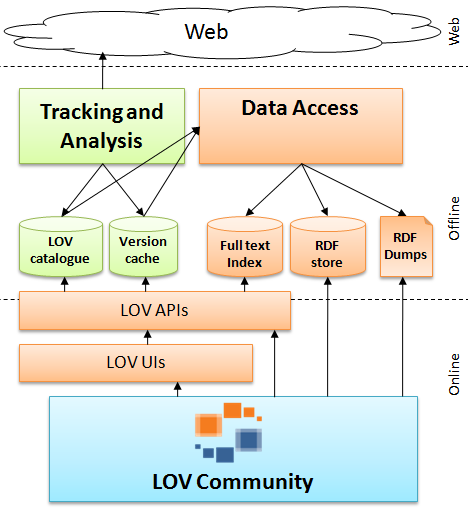
\includegraphics[scale=0.6]{lov_architecture.png}
\caption{Overview of the Linked Open Vocabularies Architecture.}
\label{fig:arch}
\end{figure}

\subsection{LOV Community}
Over the last four years, Linked Open Vocabularies initiative has gathered a community of around 350 people interested in various domain among them: ontology engineering or data publication. LOV Google+ community\footnote{\url{https://plus.google.com/communities/108509791366293651606}} is now an important place to discuss, report and announce general facts related to vocabularies on the Web. Compared to other vocabulary catalogues (cf. section \ref{sec:related}), LOV relies on a manual process for vocabulary insertion thus ensuring the quality of each vocabulary and therefore the quality of the overall LOV ecosystem. Suggestions are coming from the community and from inter-vocabulary reference links. Our system provides a feature to suggest\footnote{\url{http://lov.okfn.org/dataset/lov/suggest/}} the insertion of a new vocabulary. This feature allows a user to check what information LOV can automatically detect and extract. From our experience in vocabulary publication, we published a handbook about Metadata recommendations for linked open data vocabularies to help that process~\cite{vandenbussche2011metadata}. We consider LOV community as a core component of the system.

\subsection{Tracking and Analysis}
The vocabulary collection is maintained by curators in charge of validating\footnote{Before a vocabulary is inserted, LOV curators contact the authors to make sure the vocabulary is published following the best practices and contains enough metadata}, inserting a vocabulary in the LOV ecosystem and assigning a detailed review (updated every year). Following this manual step, the \emph{Tracking and Analysis} component takes care of dereferencing\footnote{URI is looked up over HTTP to return content in a processable format such as XML/RDF, notation 3 or turtle.} the vocabulary, storing a version locally (in notation 3 format) and extracting relevant metadata. A vocabulary consists of a collection of terms (classes and properties) expressed in W3C RDF, RDFS, OWL languages. 

At the Vocabulary level, the system extracts three types of information for each vocabulary version (figure \ref{fig:dcat}):
\begin{itemize}
\item Metadata associated to the vocabulary: this information is explicitly defined within the vocabulary to provide context, and useful data about the vocabulary. To be part of the LOV catalogue, a vocabulary must contain some minimal metadata information \cite{vandenbussche2011metadata}. Some high level vocabularies can be reused in that purpose, such as Dublin Core to describe authors, contributors, publishers or Creative Commons\footnote{\url{http://creativecommons.org/ns#}} for the description of license.

\item Inlinks vocabularies, making explicit the links to another vocabulary based on the semantic relation of their terms.

\item Outlinks vocabularies, making explicit the links from another vocabulary based on the semantic relation of their terms.
\end{itemize}

\begin{figure}[ht!b]
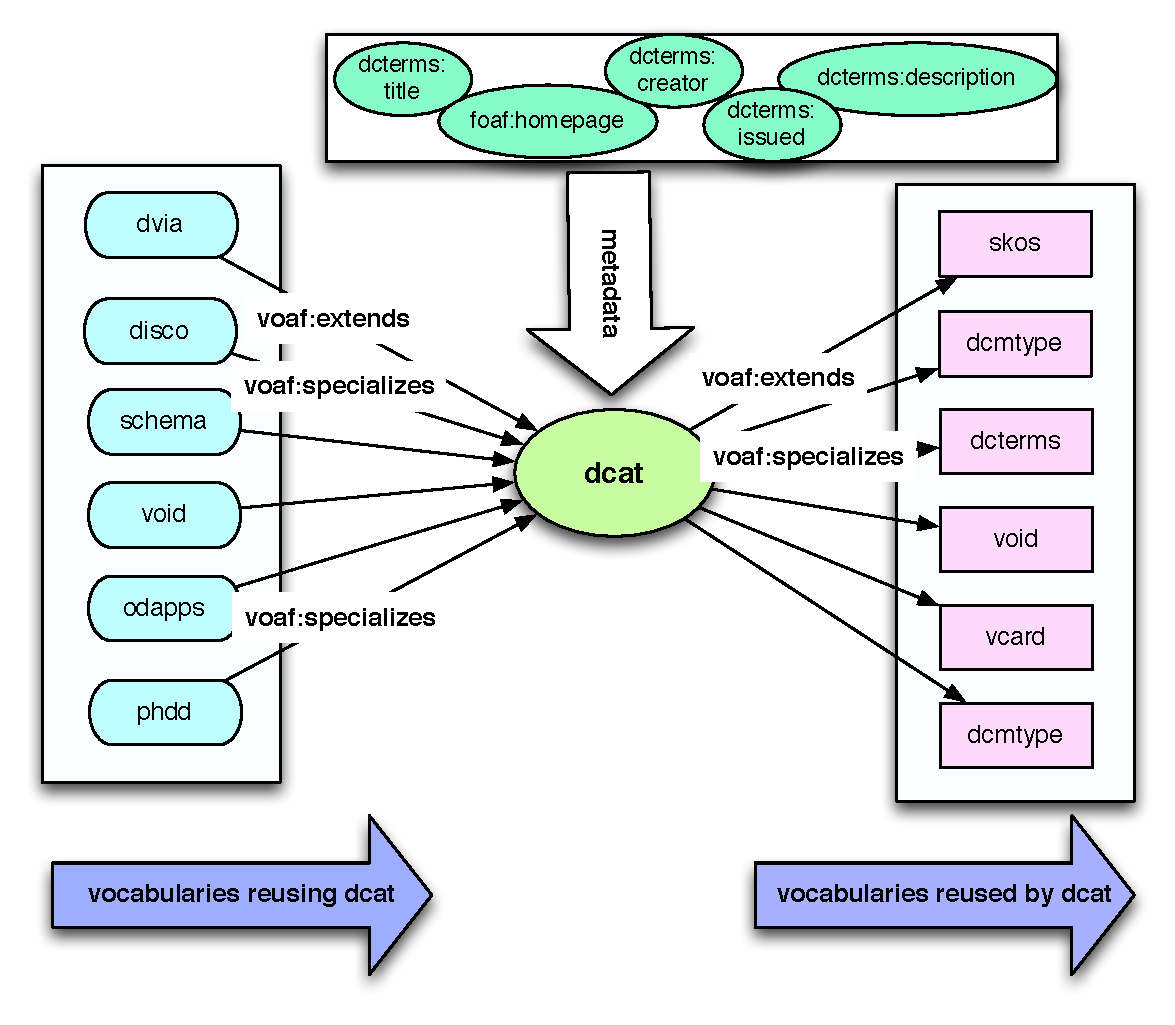
\includegraphics[scale=0.4]{dcat-relations.pdf}
\caption{Metadata type, vocabulary inlinks and outlinks of DCAT vocabulary.}
\label{fig:dcat}
\end{figure}

At the Vocabulary Term level, the system extracts labels that will be used for full text search and language information. The information of language is then inserted into LOV database at the vocabulary level using the \texttt{dcterms:language} property with the URI of the language in Library of Congress dataset using the ISO 639-2 code. For example, the URI associated to Japanese language is \url{http://id.loc.gov/vocabulary/iso639-2/jpn}. Currently, 91.25\% (428 out of 469) of vocabularies use explicitly at least one language tag, with only 9 vocabularies with labels in a language different from English. Table \ref{tab:language} presents the number and percentage of the top five languages detected in LOV. We will discuss in section \ref{sec:conclusion} the importance for publishers to provide multilingual vocabularies on the Web.
 
 \begin{table}[h!tb]
\caption{Top five languages and percentage detected in LOV catalogue.}
\begin{tabular}{lcc}
\hline
\textbf{Language} & \textbf{Number} & \textbf{\%}  \\ \hline
English  & 419   &  97.89\%      \\
French & 42 & 9.81\% \\
Spanish & 28 & 6.54\%\\
German & 21 & 4.90\%\\
Italian & 20 & 4.67\%\\
\hline  
\end{tabular}
\label{tab:language}
\end{table}

When some metadata failed to be extracted automatically (such as creators of a vocabulary), LOV curators enhance the description available in the system. The documentation provided by LOV assists any user in the task of understanding the semantic of each vocabulary term and therefore of any data using it. For instance, information about the creator and publisher is a key indication for a vocabulary user in case help or clarification is required from the author, or to assess the stability of that artifact. About 55\% of vocabularies specify at least one creator, contributor or editor. We augmented this information using manually gathered information, leading to inclusion of data about the creator in over 85\% of vocabularies in LOV. The database stores every different version of a vocabulary over time since its first issue. For each version, a user can access the file (even though the original online file is no longer available). An automatic script is in place to automatically check for vocabulary updates every day. To embrace the complexity of the vocabulary ecosystem and assess the impact of a modification, one needs to know in which vocabularies and datasets a particular vocabulary term is referenced. For the first time LOV provides such a vision. 

\subsection{Data Access}
LOV system (code and data) is published under Creative Commons 4.0 license\footnote{\url{https://creativecommons.org/licenses/by/4.0/}} (CC BY 4.0). Three methods are offered for users and applications to access LOV data:
		\begin{inparaenum}[1)] 
			\item query LOV search engine to find the most relevant vocabulary terms, vocabularies or agents matching keywords;
			\item download data dumps of the LOV catalogue in RDF Notation 3 format or the LOV catalogue and the latest version of each vocabulary in RDF N-quads format;
			\item run SPARQL queries on LOV SPARQL Endpoint;
			\item use LOV system Application Program Interfaces (APIs) which provide a full access to LOV data for software applications.
		\end{inparaenum}


\subsubsection{Search Engine}
For every vocabulary in LOV, terms (classes, properties, datatypes, instances) are indexed and a full text search feature is offered\footnote{\url{http://lov.okfn.org/dataset/lov/terms}}. Compared to other existing ontology search engines (cf. section \ref{sec:related}), the Linked Open Vocabularies search engine ranking algorithm is not only based on term popularity in datasets but take as well into account its popularity within the LOV ecosystem and most importantly assigned a different score depending on which label property a searched term matched~\cite{butt2014}. We distinguish four different label property categories on which a search term could match: 
		\begin{inparaenum}[1)] 
			\item local name (URI without the namespace). While a URI is not suppose to carry any meaning, it is a convention to use a compressed form of a term label to construct the local name. It becomes therefore an important artifact for term matching for which the highest score will be assigned. An example of local name matching the term ``person'' is \url{http://schema.org/Person}.
			\item primary labels. The highest score will also be assigned for matches on \url{rdfs:label}, \url{dce:title}, \url{dcterms:title}, \url{skos:prefLabel} properties. An example of primary label matching the term ``person'' is \url{rdfs:label} \emph{"Person"@en}.
			\item secondary labels. We define as secondary label properties: \url{rdfs:comment}, \url{dce:description},\\ \url{dcterms:description}, \url{skos:altLabel}. A medium score is assigned for matches on these properties. An example of secondary label matching the term ``person'' is \url{dcterms:description} \emph{"Examples of a Creator include a person, an organization, or a service."@en}.
			\item tertiary labels. Finally all properties not falling in the previous categories are considered as tertiary labels for which a low score is assigned. An example of tertiary label matching the term ``person'' is \url{http://metadataregistry.org/uri/profile/RegAp/name} \emph{"Person"@en}. 
		\end{inparaenum}
As a result a term matching a value for the property \url{rdfs:label} will have a higher score than if it matches a value for the property \url{dcterms:comment}. Based on the different nature of these labels, we apply different indexing tokenizers and scoring methods.

	\begin{table}[!htb]
		\caption{Two words, three words and more and URI search number in LOV.}
		\begin{tabular}{lcccc}
		\hline
		\textbf{Pattern} & \textbf{2012} & \textbf{2013} & \textbf{2014} & \textbf{Total} \\ \hline
		\textit{URI}  & 38   &  54  & 63  &  155      \\
		$t_{1}$ $t_{2}$ & 200 & 480 & 466 & 1146 \\
		($t_{1}$ $t_{2}$ $t_{3}$)* & 93 & 233 & 249 & 575\\
		\hline  
		
		\end{tabular}
		\label{tab:patterns}
	\end{table}

Human users or agents can further narrow a search by filtering on term type (class, property, datatype, instance), vocabulary domain and vocabulary. The LOV log\footnote{\url{http://lov.okfn.org/dataset/lov/stats/searchLog.csv}} of search terms between 2012/01/06 and 2014/12/09 presents a total of 54,657 terms, with 36,019 (65.90\%) duplicate terms and 18,643 unique terms (34.10\%). Figure \ref{fig:searchterms} depicts the number of terms in the log grouped by year. From 2012 to 2013, there has been an increase of more than 50\% of search in LOV. Searched terms are mostly single words (e.g., currency). However, terms can be a composition of two words (e.g., ``family tree''), three words (e.g., ``semantic sensor network'') or an URI (e.g., ``http://www.aktors.org/ontology/portal''). Table \ref{tab:patterns} details the use of URIs, two words and at least three words for unique values in the LOV search log.
	
%	\begin{figure}[!htbp]
%	\centering{
%	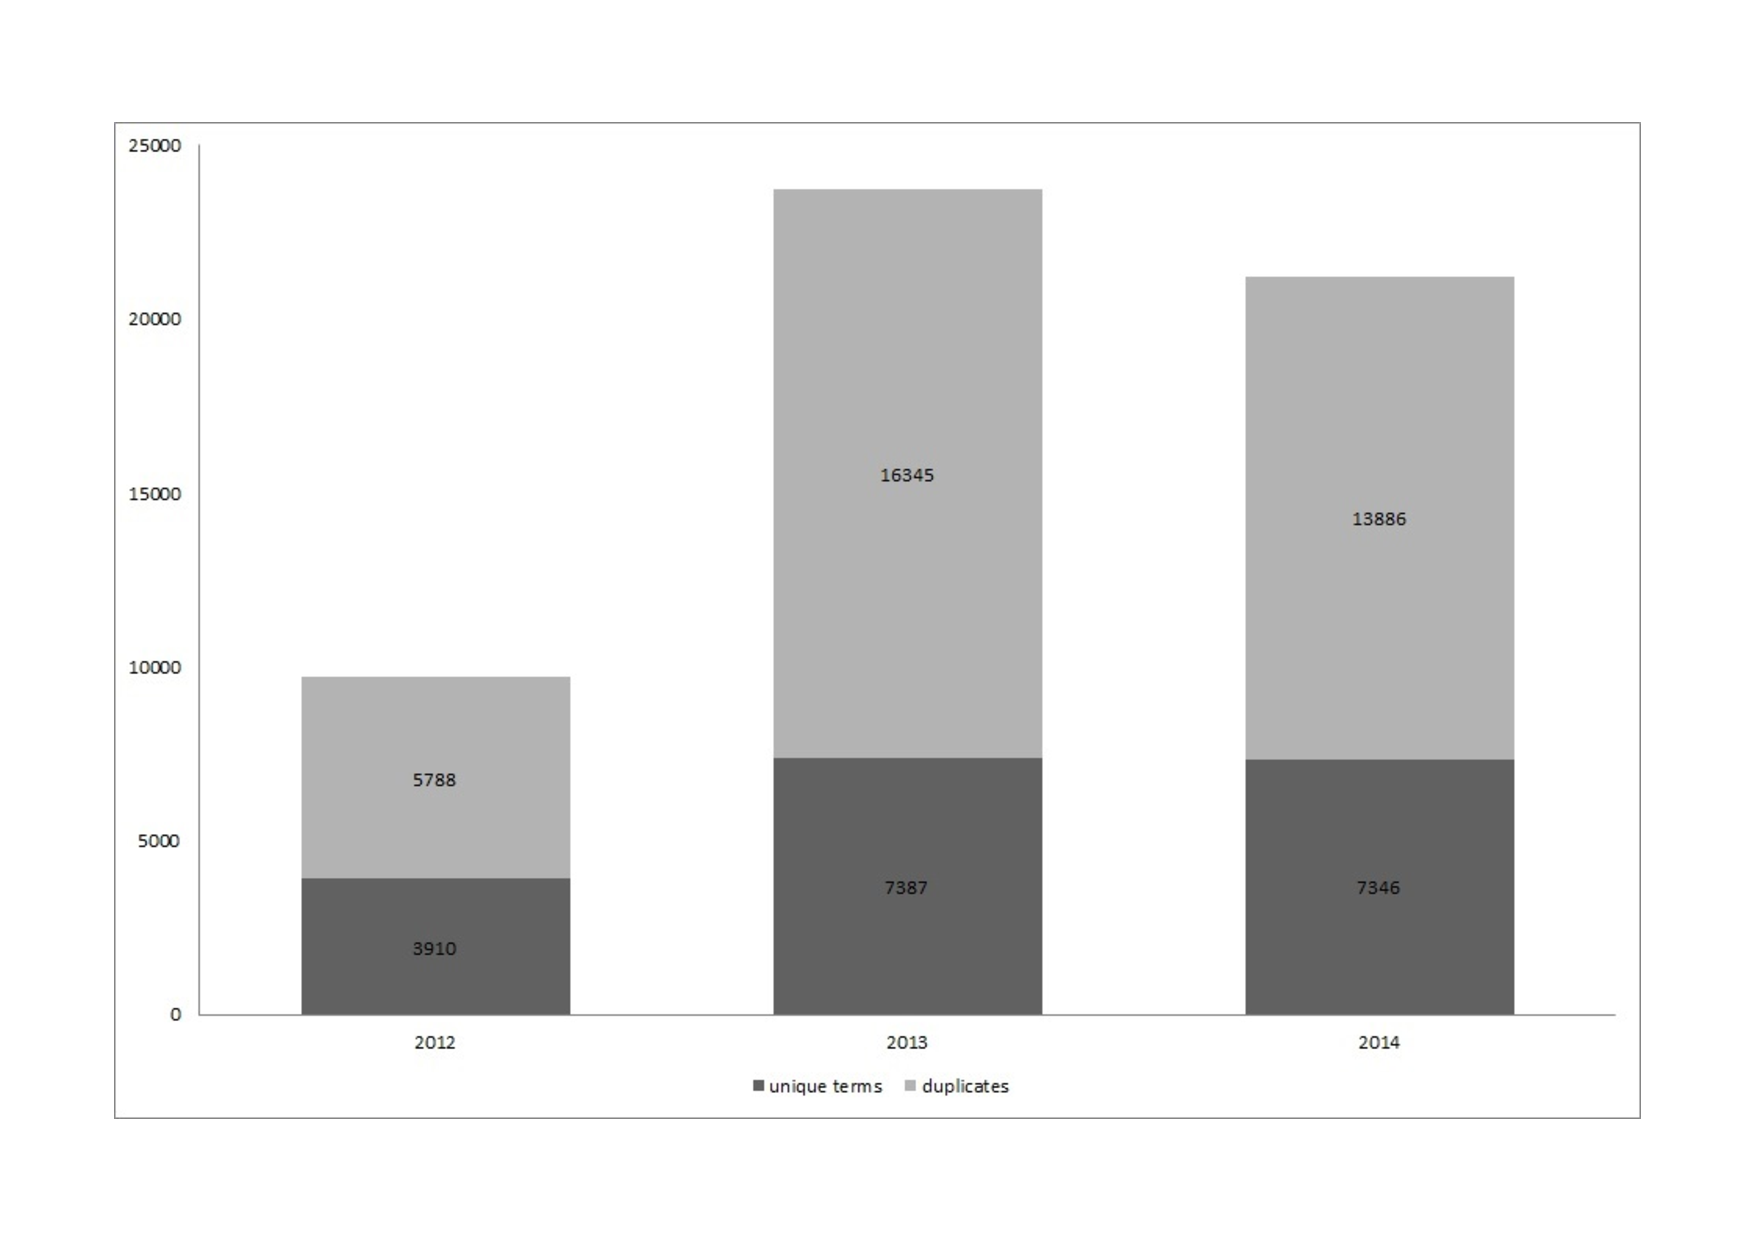
\includegraphics[scale=.28]{chart_searchterms.pdf}
%	\caption{Unique and duplicate terms searched by agents/users according to LOV log in the period between 2012/01/06 until 2014/12/09.}
%	\label{fig:searchterms}
%	}
%	\end{figure}

	\begin{figure}[tb]
	\ffigbox{
		\figfontsize%
		\begin{tikzpicture}
\begin{axis}[
legend style={at={(0.02,0.98)},anchor=north west,opacity=0.8, font=\scriptsize},
date coordinates in=x,
xticklabel={\year},
x tick label style={align=right,font=\scriptsize},
scaled ticks=false,
y tick label style={/pgf/number format/fixed},
date ZERO=2012-01-01, % Set near lowest date
xmin={2011-01-01}, 
xmax={2015-01-01},
ymin={0},
xtick={2012-01-01, % Set tick marks
2013-01-01,
2014-01-01},
grid=major,
point meta=explicit,
ybar stacked,
bar width=30pt,
every node near coord/.style={
        yshift=-15
    },
nodes near coords,
nodes near coords align=center
]


\pgfplotstableread{PGFPlots/LOVSearch.dat}\thisTable

\addplot+[black,fill=red] table[x=date,y=nbUnique, meta=nbUnique]{\thisTable};
\addlegendentry{Unique Terms}

\addplot+[black,fill=orange] table[x=date,y=nbDuplicates, meta=nbDuplicates]{\thisTable};
\addlegendentry{Duplicates}



\end{axis}
\end{tikzpicture}
	}{%
	  \caption{\label{fig:searchterms} Unique and duplicate terms searched by agents/users according to LOV log in the period between 2012/01/06 until 2014/12/09.}%
	}
	\end{figure}

\subsubsection{Data Dumps}
The system provides data dumps of the LOV vocabulary catalogue in RDF Notation 3 format and the LOV catalogue along with the latest version of each vocabulary in RDF N-quads format\footnote{\url{http://lov.okfn.org/dataset/lov/sparql}}. As illustrated in figure \ref{fig:model}, the RDF model mainly reuse the Data CATalogue Vocabulary (DCAT) which allows the representation of LOV catalogue as a \texttt{dcat:Catalog} composed of vocabulary entries (\texttt{dcat:CatalogRecord}) capturing information like the insertion date in LOV. Each entry points to the vocabulary itself represented by a sub class of \texttt{dcat:Dataset} defined in the Vocabulary of a Friend (VOAF). This artifact contains metadata extracted by LOV such as creators, first issued date, number of occurrences of the vocabulary in Linked Open datasets. Each vocabulary is then linked to its various published versions represented by the \texttt{dcat:Distribution} entity on which information such as inter vocabulary links or languages can be found.

\begin{figure*}[!htb]
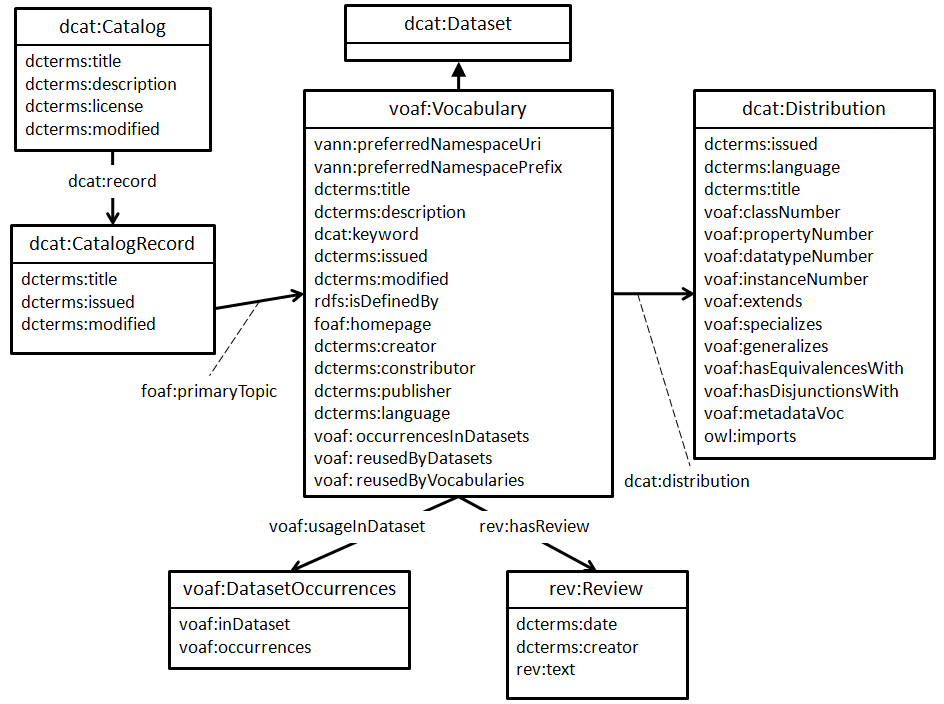
\includegraphics[scale=0.5]{model.png}
\caption{RDF representation of the LOV catalogue.}
\label{fig:model}
\end{figure*}


\subsubsection{SPARQL Endpoint}
The LOV SPARQL Endpoint offers a complementary data access method and allows clients to pose complex queries to the server and retrieve direct answers computed over the LOV dataset. We use Jena fuseki triple store to store the N-quads file containing the LOV catalogue and the latest version of each vocabulary. This allows for the first time to query multiple vocabulary at the same time and to detect inter-vocabulary dependencies. An example of this use is explained in the ontology mapping in section \ref{sec:dataPubOntoEngine}.


\subsubsection{API and UI}
LOV APIs give a remote access to the many functions of LOV through a set of Restful services\footnote{\url{http://lov.okfn.org/dataset/lov/apidoc/}}. The basic design requirements for these APIs is that they should allow applications to get access to the very same information humans do via the User Interfaces. More precisely the APIs give access, through three different type of services (cf. figure \ref{fig:apis}), to functions related to:
\begin{inparaenum}[1)] 
			\item vocabulary terms (classes, properties, datatypes and instances). With these functions, a software application can query the LOV search engine, ask for autocompletion or suggestion for misspelled terms;
			\item vocabularies. A client can get access to the current list of vocabularies contained in the LOV catalogue; search for vocabularies or get autocompletion;
			\item agents. This provides a software agent with a list of all agents references in the LOV catalogue, a mean to search for an agent and get autocompletion.
		\end{inparaenum}
LOV APIs is a convenient manner to get access to the full functionality and data of LOV. It is particularly appropriate for dynamic Web applications using scripting languages such as Javascript. The APIs described above have been developed for, and following the requirements of, Ontology design and data publication tools.

\begin{figure}[ht!b]
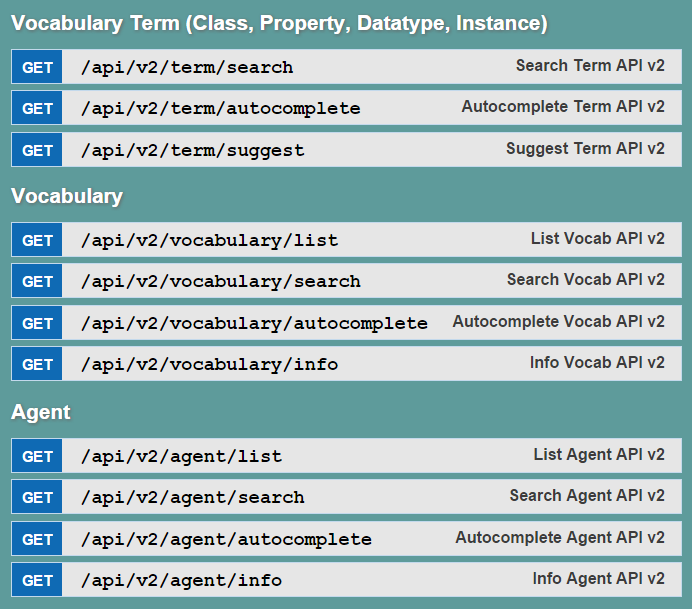
\includegraphics[scale=0.4]{apis.png}
\caption{List of APIs to access LOV data.}
\label{fig:apis}
\end{figure}

\section{LOV as a support for Data Publication and Ontology Engineering}
\label{sec:dataPubOntoEngine}


LOV can be used in any methodology for the creation and reuse of ontologies. One of the most mature methodology for supporting collaborative development of ontologies is NeOn.  
The NeOn Methodology is a scenario-based methodology that supports the collaborative aspects of ontology development and reuse, as well as the dynamic evolution of ontology networks in distributed environments. The key assets of the NeOn Methodology are \cite{MC10}:
\begin{itemize}
 \item  A set of nine scenarios for building ontologies and ontology networks, emphasizing the reuse of ontological and non-ontological resources, the re-engineering and merging, and taking into account collaboration and dynamism.
 \item The NeOn Glossary of Processes and Activities, which identifies and defines the processes and activities carried out when ontology networks are collaboratively built by teams.
 \item Methodological guidelines for different processes and activities of the ontology network development process, such as the reuse and re-engineering of ontological and non-ontological resources, the ontology requirements specification, the ontology localization, the scheduling, etc.
\end{itemize}

Based on the Neon Methodology's glossary of activities for building ontologies, LOV is relevant in four activities:

\begin{description}

 \item [Ontology Search.] Main LOV's feature is the search of vocabulary terms. These vocabularies are categorized within LOV according to the domain they address. In this way, LOV contributes to ontology search by means of (a) keyword search and (b) domain browsing.
 \item [Ontology Assessment.] LOV provides a score for each term retrieved by a keyword search. This score can be used during the assessment stage.
 \item [Ontology Mapping.] In LOV, vocabularies rely on each other in seven different ways. These relationships are explicitly stated using VOAF vocabulary\footnote{\url{http://lov.okfn.org/vocab/voaf}}. This data could be useful to find alignments between ontologies, for example one user might be interested in finding equivalent classes for a given class or all the equivalent classes among two ontologies. Listing \ref{list:alignment} shows the SPARQL query to retrieve all the equivalent classes and properties between the vocabularies \texttt{foaf} and \texttt{dcterms}\footnote{The reader can run the query on LOV Endpoint: \url{http://goo.gl/sTIGQ6}. Prefixes are omitted for readability purpose. They can be found in LOV.}.
     
 \begin{lstlisting}[basicstyle=\tiny,float=htb,caption={SPARQL query asking for all the equivalent classes and properties between the vocabularies foaf and dcterms. },label=list:alignment, language=turtle]
 PREFIX owl:<http://www.w3.org/2002/07/owl#>
 SELECT DISTINCT ?elem1 ?alignment ?elem2 {
   {?elem1 owl:equivalentClass ?elem2}
      UNION {?elem1 owl:equivalentProperty ?elem2}
      UNION {?elem2 owl:equivalentClass ?elem1}
      UNION {?elem2 owl:equivalentProperty ?elem1}
      FILTER(!isBlank(?elem2))
      FILTER(!isBlank(?elem1))
      ?elem1 ?alignment ?elem2.
      ?elem1 rdfs:isDefinedBy <http://xmlns.com/foaf/0.1/>.
      ?elem2 rdfs:isDefinedBy <http://purl.org/dc/terms/>.
 } ORDER BY ?alignment
	
	\end{lstlisting}
	
	Figure \ref{fig:eqCR} shows the alignments between foaf and dcterms vocabularies by mean of \url{owl:equivalentClass} and \\ \url{owl:equivalentProperty}.
    \begin{figure}
      \centering
      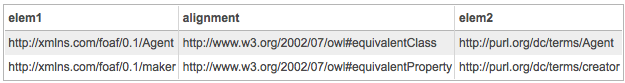
\includegraphics[width=1.0\linewidth]{equivalentCandR.png}
      \caption{Equivalent classes and properties between foaf and dcterms}
      \label{fig:eqCR}
    \end{figure}
    
 \item [Ontology Localization.] Labels in different languages are stored in the LOV endpoint. This annotations could be used when translating terms into different languages. This information could be extracted by querying the SPARQL endpoint\footnote{Result of the query can be found at the following URL: \url{http://goo.gl/JJCJ01}} as shown in Listing \ref{list:person} where all the labels defined for the terms that have at least one \url{rdfs:label} containing strictly ``person":
		
    \begin{lstlisting}[basicstyle=\tiny,float=htb,caption={SPARQL query asking all the labels defined for the terms containing person.},label=list:person, language=turtle]
 SELECT DISTINCT ?label2 ?element{
   ?element rdfs:label ?label1 .
   ?element rdfs:label ?label2 .
   FILTER (?label1 != ?label2 ).
   FILTER(REGEX(STR(?label1), "person", "i")).
 } ORDER BY ?element
	\end{lstlisting}
							
   An excerpt of the query result is shown in Figure \ref{fig:translations}. From that result, ``Persona''@es and ``Personne''@fr could be used as translations for the English term ``Person'' in Spanish and French respectively. 
   
   \begin{figure}[ht!b]
     \centering
     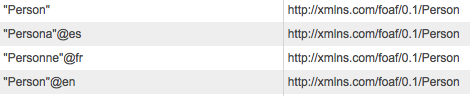
\includegraphics[width=.90\linewidth]{translations1.png}
     \caption{Translations example for foaf:Person}
     \label{fig:translations}
   \end{figure}
   
\end{description}

Figure \ref{fig:LOVandNeOn} shows the activities within the overall Neon methodologies activity workflow that can benefit from LOV.
\begin{figure}[h!tp]
\centering
  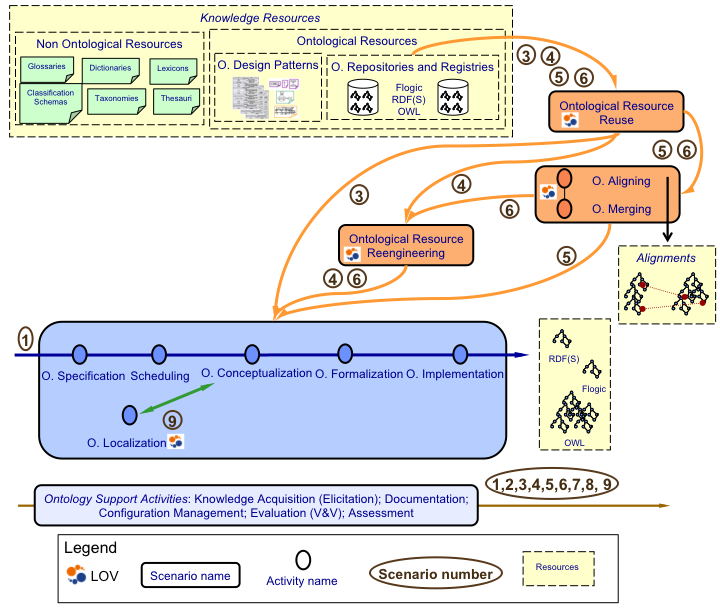
\includegraphics[width=1\linewidth]{neonScenarios.png}
  \caption{Meeting points between LOV and the NeOn methodology, derived from \cite{MC10}.}
  \label{fig:LOVandNeOn}
\end{figure}

\section{LOV application and project ecosystem}
\label{sec:lovecosystem}
As of today, LOV database contains over 46,000 RDF vocabulary terms, with 28,000 properties and 18,000 classes. LOV is supporting the emergence of a rich application ecosystem thanks to its various data access methods. We list below some tools using our system as part of their service and projects using LOV as a research artifact.
 
\subsection{Derived tools and applications}

Maguire et al. \cite{ontomaton12} uses the LOV search API to implement OntoMaton\footnote{\url{https://github.com/ISA-tools/OntoMaton}}, a widget for bringing together ontology lookup and tagging within the collaborative environment provided by Google spreadsheets. 

YASGUI (Yet Another SPARQL Query GUI)\footnote{\url{http://yasgui.laurensrietveld.nl}} is a client-side JavaScript SPARQL query editor that uses LOV API for property and class autocompletion together with \url{http://prefix.cc} for namespace prefix autocompletion \cite{yasgui}.

Datalift\footnote{\url{http://datalift.org/en/node/24}} platform \cite{scharffe_2012}, a framework for ``lifting'' raw data into RDF, comes with a module to map data objects and properties to ontology classes and predicates available in the LOV catalogue. Data2Ontology module takes an input a ``raw RDF'', that is a dataset that has been converted directly from legacy format to triples. The goal is to help to publishers reusing existing ontologies for converting their dataset for easy discovery and interlinking. It consists of three main components assisting the publisher in selecting properties suitable for the dataset to be published. 
\begin{description}
\item 1-LOV component. This component is in charge to connect with the LOV catalogue to retrieve up-to-date ontologies using the LOV search API\footnote{\url{http://lov.okfn.org/dataset/lov/apidoc/#lov2search}}.
\item 2-Matching Workflow. Data2Ontology offers to map the data to LOV by automatically proposing a list of best matches.
\item 3-SPARQL Generator. This module receives as input the desired mappings and creates the SPARQL CONSTRUCT query needed to implement the mapping. The query can further be modified before the execution to generate a new dataset in the lifting process with Datalift.
\end{description}

OntoWiki\footnote{\url{http://ontowiki.net/}} facilitates the visual presentation of a knowledge base as an information map, with different views on instance data \cite{auer2006ontowiki}. It enables intuitive authoring of semantic content, with an inline editing mode for editing RDF content, similar to WYSIWIG for text documents. OntoWiki offers a vocabulary selection feature based on LOV.

\subsection{Using LOV as a Research platform}
%\maria{ write input of your work on onto pitfalls using LOV dataset }. \\

LOV vocabularies have served as object of study in \cite{poveda2012landscape} where trends in ontology reuse techniques were analyzed in 2012. In addition, LOV dataset has been used in order to analyze the occurrence of good and bad practices in vocabularies as described in \cite{poveda2013detecting} in 2013.

Prefixes in LOV dataset is regularly mapped with namespaces in the prefix.cc service. In \cite{wasabi13}, the authors performs alignments of Qnames of vocabularies in both services, and provides different solutions to handle in case of clashes and disagreements on preferred namespaces. Both LOV and prefix.cc provide associations between prefixes and namespaces but following a different logic. The prefix.cc service supports polysemy and synonymy, and has a very loose control on its crowd-sourced information. In contrast, LOV has a much more strict policy forbidding polysemy and synonymy ensuring that each vocabulary in the LOV database is uniquely identified by a unique prefix identification allowing the usage of prefixes in various LOV publication URIs. This requirement leads sometimes to a situation where LOV uses prefixes differently from the ones recommended by the vocabulary publishers.

LOV query log covering the period between 06/01/2012 and 16/04/2014 is used in \cite{butt2014} to build a benchmark suite for ontology search and ranking. The CBRBench\footnote{\url{https://zenodo.org/record/11121}} benchmark uses eight ranking models of resources in ontologies and compare the results with ontology engineers. We plan to start a collaboration with the authors to enhance LOV search based on the study result.

In \cite{janowicz2014five}, the authors rate vocabularies according to some criteria beyond the sameAs links but subClassOf and equivalentClass 'links' between vocabularies to foster interoperability, query federation, ease the interpretation of data, and so forth. %\ghis{ read this paper to add more content here}

Databugger\footnote{\url{https://github.com/AKSW/Databugger}} is a test-driven data debugging framework for the Web of Data. In \cite{databugger,rdfunit}, the authors provide an automatic test case instantiations for all available schemata registered with LOV. In this case, the vocabularies of LOV are used to encode semantics to domain specific knowledge to check the quality of data.

Giovanni et al. \cite{governatori2014} analyzes the current use of licenses in vocabularies on the Web based on LOV catalogue to further propose a framework to detect incompatibilities between datasets and vocabularies.


\section{Related work and Discussion}
\label{sec:related}

Reusing vocabularies requires searching for terms in existing specialized vocabulary catalogues or search engines on the web. While we refer the reader to~\cite{AquinJoWS12} for a systematic survey of ontology repositories, we list below some existing catalogues relevant to find vocabularies \cite{wasabi13}:
\begin{itemize}
 \item \textit{Catalogs of generic vocabularies/schemas} similar to LOV catalogue. Example of catalogues falling in this category are vocab.org\footnote{\url{http://vocab.org/}}, ontologi.es\footnote{\url{http://ontologi.es/}}, JoinUp Semantic Assets or the Open Metadata Registry.
 \item \textit{Catalogs of ontologies for a specific domain} such as biomedicine with the BioPortal \cite{bioportal11}, geospatial ontologies with SOCoP+OOR\footnote{\url{http://socop.oor.net/}}, Marine Metadata Interoperability and the SWEET \cite{sweet05} ontologies\footnote{\url{http://sweet.jpl.nasa.gov/2.1/}}. The SWEET ontologies include several thousand terms, spanning a broad extent of Earth system science and related concepts (such as data characteristics), with the search tool to aid finding science data resources. 
 \item \textit{Catalogs of ontology Design Patterns (ODP)} focused on reusable patterns in ontology engineering \cite{presutti08}. The submitted patterns are small pieces of vocabularies that can further be integrated or linked with others vocabularies. ODP is more targeted on  reusable successful solution to a recurrent modeling problem. However, it does not provide a search function for specific terms as it is the case with Swoogle or Watson.
 \item \textit{Search Engines of ontology terms}. Among ontology search engines, we can cite: Swoogle \cite{finin2005swoogle}, Watson \cite{d2007watson,Sabou07} and FalconS \cite{cheng2008falcons}. These search engines crawl for data schema from RDF document on the Web. They offer a filtering based on ontology type (Class, Property) and a ranking based on the popularity. They don't look for ontology relations nor check if the definition of the ontology is available (usually known as dereferenciation)
\end{itemize}


LOV focuses only on vocabularies (subpart of semantic documents of the web) submitted by any user, reviewed and validated by curators. In addition, LOV keeps track of different versions of the vocabularies in the server that can be retrieved for comparing the differences between along the time evolution.  In contrast, Swoogle is designed to automatically discover Semantic Web Documents (SWDs), indexes their metadata and answers queries about it. Thus, the result of a search query retrieved any semantic document. For example, a query of the term \textit{person} gives $16,438$ results while in LOV, the term only appears in $134$ vocabularies.
Watson works similarly to Swoogle, crawling and indexing semantic document at a small scale, explicitly distinguishing for each document (resource), concepts, properties and individuals if available. While in Swoogle  the ranking score is displayed, Watson shows the language of the resource and the size. Falcons is a keyword-based search system for concepts and objects on the Semantic Web, and is equipped with entity summarization for browsing. It is notable that Falcons limits the search only to ontologies and a recommendation feature is provided according to users' preferences. However, it does not provide any relationships between the related ontologies, nor any domain classification of the vocabularies.
Table \ref{tab:lovfeatures} compares key features of LOV with respect to Swoogle, Watson and Falcons.
 \begin{table*}[!htb]
\centering{
\begin{tabular}{lllll}
\hline
 \textbf{Feature}	& Swoogle & Watson & Falcons & LOV 			 \\ \hline
Browsing ontologies	   & Yes & Yes & Yes & Yes \\
Ontology Discovery Method   & Automatic & Automatic & Automatic & Manual \\
Scope & SWDs & SWDs & Concepts & Ontologies \\
Ranking	& LOD popularity & LOD popularity & LOD popularity &  LOD/LOV popularity\\
&&&&+ property semantic score	 \\
Domain filtering & No & No & No & Yes \\
Comments and review 	& No & Yes & No & Only by curators	\\
Web service access & Yes & Yes & Yes & Yes		\\
SPARQL endpoint	& No & No & No & Yes		\\
Read/Write	& Read & Read \& Write & Read &Read  	\\
Ontology directory & No & No & No &Yes \\
Application platform & No & No & No & Yes \\
Storage & Cache & - & - & Dump \& endpoint \\
Interaction with Contributors & No &  - & No & Yes \\

		\\ \hline

\end{tabular}
\caption{Comparison of LOV, with respect to Swoogle, Watson and Falcons; based on part of the framework defined in \cite{AquinJoWS12}.  }
\label{tab:lovfeatures}
}
\end{table*}

LOV search engine is to the best of our knowledge, the only purpose-built ontology search engine available on the Web with an up-to-date index.

\section{Conclusion and Future work}
\label{sec:conclusion}
In this system report, we presented an overview of the Linked Open Vocabularies initiative. The importance of this work is motivated by the difficulty for data publishers to determine which vocabularies to use to describe their data. The key innovations described in this article include: 
\begin{inparaenum}[1)] 
	\item the availability of a high quality vocabularies dataset through multiple accessing methods,
	\item the vocabulary metadata curation by experts, making explicit for the first time the relationships between vocabularies and their version history,
	\item the consideration of property semantic in term search scoring.
\end{inparaenum}

The adoption and integration of the LOV catalogue in applications for vocabulary engineering, reuse and data quality are significant. Linked Open Vocabularies has a central role in vocabulary life-cycle on the Web of Data. In the future, we see in particular the following directions for advancing the LOV initiative:

\emph{From single to multi-term search.} An area which is still largely unexplored is multi-term vocabulary search. During the ontology design process, it is common to have more than 20 concepts to be represented using existing vocabularies or a new one in case there is no corresponding artifact. When we are able to search for relevant terms in LOV it is still the responsibility of the ontology designer to understand the complex relationships betwen all these terms and come up with a coherent ontology. We could use the network of vocabularies defined in LOV to suggest not only terms result but graphs to represent several concepts together.

\emph{Multilingual vocabularies.} There is a need for vocabularies to support more languages. Labels are the main entrypoint to a vocabulary and their associated language is the key. Only 18\% of LOV vocabularies use a different language than English. Multilingualism is important at least for two reasons: 
\begin{inparaenum}[1)] 
	\item the most obvious one is allowing users to search, query and navigate vocabularies in their native language,
	\item translating is a process through which the quality of a vocabulary can only improve. Looking at a vocabulary through the eyes of other languages and identifying the difficulties of translation helps to better outline the initial concepts and if necessary refine or revise them. 
\end{inparaenum} 
Hence multilingualism and translation should be native, built-in features of any vocabulary construction, not a marginal task.

\emph{Query extension and rewriting.} Another research perspective is SPARQL query extension and rewriting based on Linked Vocabularies. Using the inter-vocabulary relationships we could transform the query to use the same semantic (same vocabulary terms) as the data source(s) to query.

\section*{Acknowledgments}
This work has been partially supported by the French National Research Agency (ANR) within the Datalift Project, under grant number ANR-10-CORD-009 and the Spanish project BabelData (TIN2010-17550) and Fujitsu Laboratories. The Linked Open Vocabularies initiative is graciously hosted by the Open Knowledge Foundation. Thanks to all the members of the LOV community in Google+\footnote{\url{https://plus.google.com/communities/108509791366293651606}}, all the editors and publishers of vocabularies who trust in the LOV catalogue. 


\bibliographystyle{plain}
\bibliography{lov}
\end{document}
